\documentclass[11pt]{article}
\usepackage[margin=0.8in]{geometry}
\usepackage[]{amsfonts, amssymb, amsmath, float, hyperref,fancyheadings, graphicx, derivative}
\pagestyle{fancy}
\lhead{Design and Analysis of Algorithms}
\chead{Larry128}
\rhead{COMP3711}
\renewcommand{\footrulewidth}{0.4pt}
\setcounter{tocdepth}{3} % set TOC
\newcommand{\indep}{\perp \!\!\! \perp}

% codeblocks
\usepackage{listings}
\usepackage{xcolor}
\definecolor{codegreen}{rgb}{0,0.6,0}
\definecolor{codegray}{rgb}{0.5,0.5,0.5}
\definecolor{codepurple}{rgb}{0.58,0,0.82}
\definecolor{backcolour}{rgb}{0.95,0.95,0.92}
\lstdefinestyle{mystyle}{
    backgroundcolor=\color{backcolour},   
    commentstyle=\color{codegreen},
    keywordstyle=\color{magenta},
    numberstyle=\tiny\color{codegray},
    stringstyle=\color{codepurple},
    basicstyle=\ttfamily\footnotesize,
    breakatwhitespace=false,         
    breaklines=true,                 
    captionpos=b,                    
    keepspaces=true,                 
    numbers=left,                    
    numbersep=5pt,                  
    showspaces=false,                
    showstringspaces=false,
    showtabs=false,                  
    tabsize=3
}
\lstset{style=mystyle}
\lstdefinestyle{customc}{
  language=C++,
  % Add other settings here
}

%common math symbols
\newcommand{\R}{\mathbb{R}}
\newcommand{\N}{\mathbb{N}}
\newcommand{\Q}{\mathbb{Q}}
\newcommand{\ddx}{\dfrac{d}{dx}}


% asymptotic notations
\newcommand\BigO[1]{$O($#1$)$}
\newcommand\BigOmega[1]{$\Omega($#1$)$}
\newcommand\BigTheta[1]{$\Theta($#1$)$}

% pgfplots
\usepackage{pgfplots}
\pgfplotsset{compat=1.18, width=8cm}
\usepackage{geometry}
\geometry{
a4paper,
total={170mm,257mm},
left=20mm,
top=20mm,
}

\begin{document}
\begin{titlepage}
    \begin{center}
        \vspace*{1cm}
            
        \Huge
        \textbf{COMP3711}
            
        \vspace{0.5cm}
        \LARGE
        Design and Analysis of Algorithms
            
        \vspace{1.5cm}
            
        Larry128
            
        \vfill
            
        A summary notes for revision
            
        \vspace{0.8cm}
                
        \Large
        Fall 2024-2025
            
    \end{center}
\end{titlepage}

\tableofcontents
\newpage


\section{Prerequisites}
\subsection{Input size of Problems}

\begin{tabular}{ll}
\textbf{Input size}& how large the input is.\\
\textbf{Assumption}& 1. any number can be stored in a computer word\\
&2. each arithmetic operation takes constant time\\
\textbf{Examples}& Sorting: Size of the list or array\\
& Graph problems: Numbers of vertices and edges\\
& Searching: Number of input keys
\end{tabular}

\subsection{Asymptotic Notation}

\begin{enumerate}
\item Running time/ Cost of algorithms\\
\begin{tabular}{l}
 i. a function of input size: $T(n)$\\
 ii. number of operations (e.g., comparisons between two numbers)\\
 iii. using \textbf{asymptotic notation}, which ignores constants and non-dominant growth terms
\end{tabular}

\item Intuitions\\
\begin{tikzpicture}[scale= 0.05]
\draw [-latex](-10, 0) -- (100, 0) node[right]{$n$};
\draw [-latex](0, -10) -- (0, 100) node[left]{$T(n)$};
\draw [red] plot [smooth, tension=1] coordinates {(20,20) (30,20) (40,25) (50,30)(60, 35) (70,40) (80, 50)(90, 60)} node[right]{Algorithm 1};
\draw [blue] plot [smooth, tension=1] coordinates {(20,10) (30,15) (40,35) (50,50)(60, 60) (70,70) (80, 80)(90, 90)} node[left]{Algorithm 2};
\end{tikzpicture}\\
From the figure above, Algorithm 2 is better for large $n$.\\

\item Rigorous definition of asymptotic notation\\
\begin{tabular}{|c|l|}
\hline
Upper bound $T(n) = O(f(n))$& if $\exists c > 0$ and $n_0 \geq 0$ such that $\forall n \neq n_0 , T(n) \leq c f(n)$\\
\hline
Lower bound $T(n) = \Omega(f(n))$& if $\exists c > 0$ and $n_0 \neq 0$ such that $\forall n \neq n_0 , T(n) \geq c f(n)$\\
\hline
Tight bound $T(n) = \Theta(f(n))$& if $T(n) = O(f(n))$ and $T(n) = \Omega(f(n))$\\
\hline
\end{tabular}

\item Big-O Notation\\
\begin{tikzpicture}[scale= 0.05]
\draw [-latex](-10, 0) -- (100, 0) node[right]{$n$};
\draw [-latex](0, -10) -- (0, 100) node[left]{$T(n)$};
\draw [red] (0, 0) -- (100, 100) node[left]{$c \cdot g(n)$};
\draw [blue] plot [smooth, tension = 1] coordinates{(0, 10) (20, 20) (30, 25) (40, 28) (50, 31) (60, 35) (70, 39) (80, 45)} node[right]{$T(n)$};
\draw [dotted] (20, 20) -- (20, 0) node[below]{$n_{0}$};
\end{tikzpicture}
$$T(n)= O(g(n)) \iff \exists n_{0} > 0 \text{ s.t. } \forall n \geq n_0, 0 \leq T(n) \leq c \cdot g(n)$$
Below are some examples of Big-O notation proofs
\begin{enumerate}
\item $T(n) = n, g(n) = n \log_{2} n$\\
We wish to proof $T(n) = n \in O(n \log_2 n)$.\\
Choose $c = 1, n_{0} = 2$, for all $n \geq 2 = n_0$, 
$$1 \leq \log_2 n \iff n \leq n \log_2 n \iff n \leq c \cdot n \log_2 n$$
\begin{center}
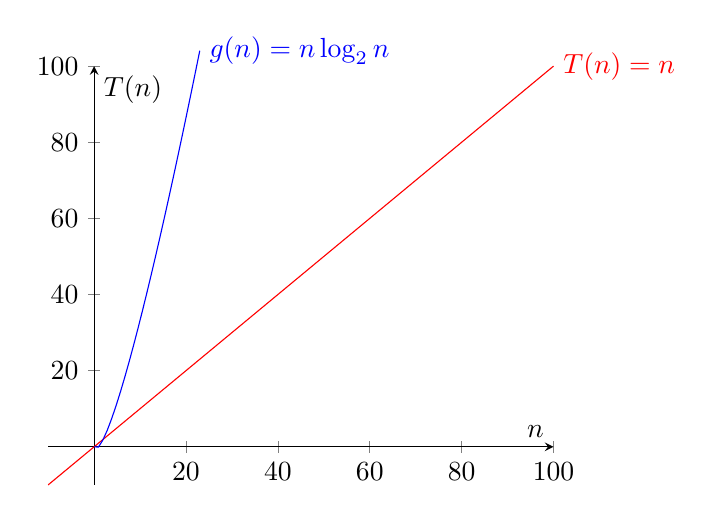
\begin{tikzpicture} [scale = 1]
\begin{axis}[clip = false,
axis lines= middle,
xmin = -10,
xmax = 100,
ymin= -10,
ymax = 100,
xlabel = {$n$},
ylabel = {$T(n)$}]
\addplot[domain = -10:100, color = red]{x}{node[right]{$T(n) = n$}};
\addplot[domain = 0:23, color = blue]{x*log2 x}{node[right]{$g(n) = n \log_2 n$}};
\end{axis}
\end{tikzpicture}
\end{center}
\item $T(n) = n^2, g(n) = n$\\
We wish to proof $T(n) = n^2 \not \in O(g(n))$ by contradiction.\\
Suppose there exists some $c$ and $n_0$ such that for all $n \geq n_0$, $n^2 \leq c \cdot n$. Then, $n \leq c$, $\forall n \geq n_0$, which is not possible as $c$ is a constant and $n$ can be arbitrarily large.
\begin{center}
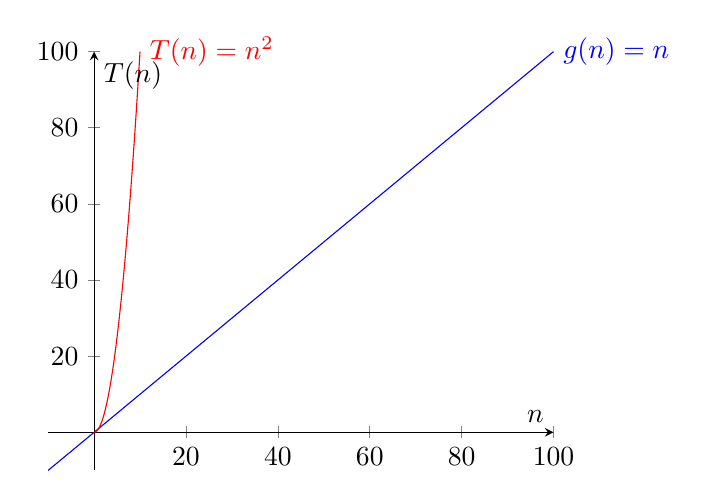
\begin{tikzpicture} [scale = 1]
\begin{axis}[clip = false,
axis lines= middle,
xmin = -10,
xmax = 100,
ymin= -10,
ymax = 100,
xlabel = {$n$},
ylabel = {$T(n)$}]
\addplot[domain = -10:100, color = blue]{x}{node[right]{$g(n) = n$}};
\addplot[domain = 0:10, color = red]{x^2}{node[right]{$T(n) = n^2$}};
\end{axis}
\end{tikzpicture}
\end{center}
\end{enumerate}
\item Big-$\Omega$ Notation\\
\begin{tikzpicture}[scale= 0.05]
\draw [-latex](-10, 0) -- (100, 0) node[right]{$n$};
\draw [-latex](0, -10) -- (0, 100) node[left]{$T(n)$};
\draw [red] (0, 20) -- (100, 30) node[left]{$c \cdot g(n)$};
\draw [blue] plot [smooth, tension = 1] coordinates{(0, 10) (20, 20) (30, 25) (40, 28) (50, 31) (60, 35) (70, 39) (80, 45)} node[right]{$T(n)$};
\draw [dotted] (25, 23) -- (25, 0) node[below]{$n_{0}$};
\end{tikzpicture}
$$T(n)= \Omega(g(n)) \iff \exists n_{0} > 0 \text{ s.t. } \forall n \geq n_0, 0 \leq c \cdot g(n) \leq T(n)$$
\\
\item Big-$\Theta$ Notation\\
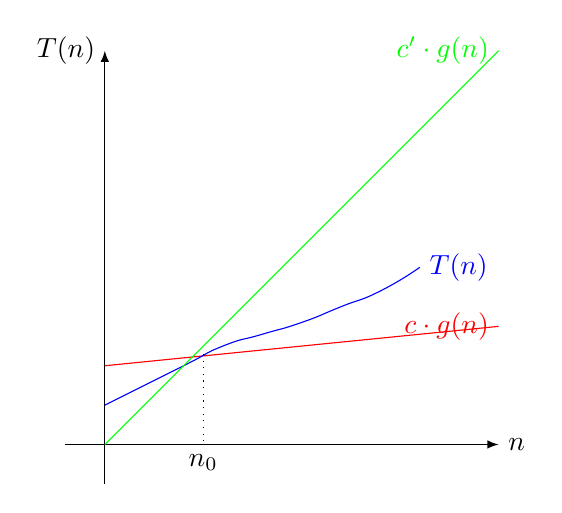
\begin{tikzpicture}[scale= 0.05]
\draw [-latex](-10, 0) -- (100, 0) node[right]{$n$};
\draw [-latex](0, -10) -- (0, 100) node[left]{$T(n)$};
\draw [red] (0, 20) -- (100, 30) node[left]{$c \cdot g(n)$};
\draw [blue] plot [smooth, tension = 1] coordinates{(0, 10) (20, 20) (30, 25) (40, 28) (50, 31) (60, 35) (70, 39) (80, 45)} node[right]{$T(n)$};
\draw [green] (0, 0) -- (100, 100) node[left]{$c' \cdot g(n)$};
\draw [dotted] (25, 23) -- (25, 0) node[below]{$n_{0}$};
\end{tikzpicture}
$$T(n) = \Theta(f(n)) \iff T(n) = O(f(n)) \text{ and }T(n) = \Omega(f(n))$$

\item Implementation and experimentation are needed sometimes\\
If algorithm A is $T_1 (n) = 10n \in \Theta(n)$, algorithm B is $T_2 (n) = 1000n \in \Theta(n)$, but algorithm A is superior in practice. In this case, Implementation and experimentation are needed.

\item Basic facts on exponents and logarithms
\begin{enumerate}
\item $2^{2n} \neq \Theta (2^n)$, proof: set $x=2^n$, then $x^2 \neq \Theta (x)$
\item $2^{n+2} = 4 \cdot 2^n = \Theta (2^n)$
\item $\log_a(n^b) = \dfrac{b \log n}{\log a} = \Theta (\log n)$
\item $\log_{b} a = \dfrac{1}{\log_{a} b}$
\item $a^{\log_{b} n} = n^{\log_{b} a}$
\end{enumerate}

\item Important note on growth of functions
$$k < \log n < n^{a} < n \log n < n^{b} < c^{n}$$
,where $k, c \in \R , 0 < a < 2, b \geq 2 \text{ are constants}$
\begin{enumerate}
\item $999^{999^{999}} = \Theta (1)$
\item $\log \log n = O(\log n)$, proof: for $n \geq 2$, $\log \log n \leq \log n$\\
\begin{tikzpicture} [scale = 1]
\begin{axis}[clip = false,
axis lines= middle,
xmin = -10,
xmax = 100,
ymin= -2,
ymax = 6,
xlabel = {$n$},
ylabel = {$T(n)$}]
\addplot[domain = 0:100, color = red]{log10 x}{node[right]{$\log x$}};
\addplot[domain = 0:100, color = blue]{log10 log10 x}{node[right]{$\log \log x$}};
\end{axis}
\end{tikzpicture}
\item $n \log n = O(\dfrac{n^2}{\log n})$\\
proof: To show $n \log n = O(\dfrac{n^2}{\log n})$, it suffices to show that there exists a $C > 0$, such that $n \log n < C \cdot \dfrac{n^2}{\log n}$ for sufficiently large $n$.
\begin{align*}
& n \log n  < C \cdot \dfrac{n^2}{\log n}\\
\iff & (\log n)^2 < C \cdot n
\end{align*}
It's obvious that for large $n$, $\log (n) < n^{\epsilon}$ for $\epsilon > 0$, then we can pick $\epsilon =  \dfrac{1}{2}$
\begin{align*}
\log n < n^{\frac{1}{2}}\\
(\log n) ^2 < n
\end{align*}
Since $C > 0$, we can see $(\log n) ^2 < n < C \cdot n$. We are done.
\end{enumerate}

\item Extra Examples
\begin{enumerate}
\item $1000n + n \log n = O(n \log n)$
\item $n^2 + n \log (n^3) = n^2 + 3n \log n = O(n^2)$
\item $n ^3 = \Omega (n)$
\item $n^3 = O(n ^{10})$
\item Let $f(n)$ and $g(n)$ be non-negative functions. Using basic definition of $\Theta$-notation, proof that $\max\{f(n), g(n)\} = \Theta(f(n) + g(n))$
\begin{enumerate}
\item Step 1: proof $\max \{ f(n), g(n)\} = O(f(n) + g(n))$\\
For all $n$, $\max \{ f(n), g(n)\}$ is either equal to $f(n)$ or equal to $g(n)$. So we can deduce that $\max \{ f(n), g(n)\} \leq f(n) + g(n)$. Therefore, $\max \{ f(n), g(n)\} = O(f(n) + g(n))$.
\item Step 2: proof $\max \{ f(n), g(n)\} = \Omega(f(n) + g(n))$\\
Note that $\max \{ f(n), g(n)\} \geq f(n)$ and $\max \{ f(n), g(n)\} \geq g(n)$. So 
\begin{align*}
\max \{ f(n), g(n)\} + \max \{ f(n), g(n)\} \geq f(n) + g(n) \\
2\cdot \max \{ f(n), g(n)\} \geq f(n) + g(n)\\
\max \{ f(n), g(n)\} \geq \frac{1}{2} (f(n) + g(n))
\end{align*}
Then, we have $\max \{ f(n), g(n)\} = \Omega (f(n) + g(n))$
\end{enumerate}
\item if $A = \log \sqrt{n}, B = \sqrt{\log n}$, then $A = \Omega(B)$\\
proof: $A = \log \sqrt{n} = \dfrac{1}{2} \log n = \Theta(\log n)$, $B = \sqrt{\log n} = \Theta(\log n)$. We can simply deduce that $\log \sqrt{n} = \Omega(\sqrt{\log n})$
\item Bounds of series - Arithmetic Series\\
Proof that $\sum_{i=1}^{n} i = 1 +2 +3 + \cdots + (n-1) + n = \Theta (n^2)$
\begin{enumerate}
\item Approach 1: use formula $\sum_{i=1}^{n} i = \dfrac{n(1+n)}{2} = \Theta (n^2)$
\item Approach 2
\begin{enumerate}
\item Step 1: proof $\sum_{i=1}^{n} i = O(n^2)$\\
\begin{align*}
\sum_{i=1}^{n} i &= 1 +2 +3 + \cdots + (n-1) + n\\
& \leq n + n + ... + n\\
& = \sum_{i=1}^{n} n\\
& = n \cdot n \\
& = n^2 =O(n^{n})
\end{align*}
\item Step 2: proof $\sum_{i=1}^{n} i = \Omega(n^2)$
\begin{align*}
\sum_{i=1}^{n} i &= 1 +2 +3 + \cdots + (n-1) + n\\
& \geq 0+ 0 + \cdots + 0 +...+ \frac{n}{2} + (\frac{n}{2} +1) + \cdots +n \\
& \geq \frac{n}{2} \cdot \frac{n}{2} \\
& = \frac{n^2}{4} = \Omega(n^2)
\end{align*}
\end{enumerate}
Then, we can say that $\sum_{i=1}^{n} i = \Theta (n^2)$
\end{enumerate}
\item Bounds of series - Polynomial Series\\
Proof that $\sum_{i=1}^{n} i^{c} = 1^c +2^c +3^c + \cdots + (n-1)^c + n^c = \Theta (n^{c+1})$\\
(The proof is more or less the same as the approach 2 of arithmetic series.)
\item Bounds of series - Harmonic Series $H_n$\\
Proof that $H_{n} = \sum_{i=1}^{n} \frac{1}{i} = \Theta(\log n)$.\\
Let $k = \log_2 n$, then $n = 2^k$. \\
\begin{tabular}{|l|l|l|l|}
\hline
index&lower bound& parts of $H_n$& upper bound\\
\hline
0&$\dfrac{1}{2}$& $1$& $1$\\
\hline
1&$2 \times \dfrac{1}{4} = \dfrac{1}{2}$ &$\dfrac{1}{2}+ \dfrac{1}{3}$& $2 \times \dfrac{1}{2} = 1$\\
\hline
2&$4 \times \dfrac{1}{8} = \dfrac{1}{2}$ &$\dfrac{1}{4}+ \dfrac{1}{5}+ \dfrac{1}{6}+ \dfrac{1}{7}$& $4 \times \dfrac{1}{4} = 1$\\
\hline
&$\cdots$ & $\cdots$ & $\cdots$\\
\hline
k-1&$2^{k-1} \times \dfrac{1}{2^k} = \dfrac{1}{2}$ &$\dfrac{1}{2^{k-1}}+\dfrac{1}{2^{k-1}+1} \cdots +\dfrac{1}{2^{k} -1}$& $2^{k-1} \times \dfrac{1}{2^{k-1}} = 1$\\
\hline
k&$0$& $\dfrac{1}{2^k} = \dfrac{1}{n}$& 1\\
\hline
\end{tabular}\\\\
Therefore, $H_n < \sum_{i=0}^{k} 1 = k +1 = \log_2 n +1 = O(\log n)$ and $H_n > \sum_{i=0}^{k-1} \dfrac{1}{2} +0 = \dfrac{k}{2} = \frac{\log_2 n}{2} = \Omega (\log n)$. So, $H_{n} = \sum_{i=1}^{n} \frac{1}{i} = \Theta(\log n)$.
\end{enumerate}
\end{enumerate}

\subsection{Introduction to Algorithms}
\begin{enumerate}
\item What is an algorithm?\\
An algorithm is an explicit, precise, unambiguous, mechanically-executable sequence of elementary instructions.
\item Examples of algorithms
\begin{enumerate}
\item adding two numbers\\
Input: 2 numbers $x = \overline{x_{n} x_{n-1} \cdots x_{1}}, y = \overline{y_{n} y_{n-1} \cdots y_{1}}$.\\
Output: A number $z= \overline{z_{n+1} z_{n} \cdots z_{1}}$, such that $z = x+y$.
\begin{lstlisting}[language = C++]
/*We assume x, y are arrays of length n, z is of length n+1 */
int c = 0; // offset
for (int i = 0; i < n; ++i){
	z[i] = x[i] + y[i] + c;
	if (z[i] >= 10) {
		c = 1;
		z[i] = z[i] - 10;	
	}else c = 0;
}
z[n] = c;
\end{lstlisting}
\end{enumerate}
\end{enumerate}
\end{document}